%%
%% Berliner Hochschule für Technik --  Abschlussarbeit
%%
%% Chapter 1
%%
%%

\chapter{First section}

The first section is intended to be a \index{user manual}.   This example document of a thesis shows all the possibilities that can be realized with the style \texttt{bhtThesis.sty}.  This does not mean that all functionalities must necessarily be used in all theses.

\section{Prerequisites}
Of course, this document also uses other \LaTeX packages. Should be available on your system:

\begin{itemize}
\item \texttt{ifthen}:  Internal use for queries
\item \texttt{graphicx}: 
  Integration of graphics
\item \texttt{array, tabularx}                  
  Table extensions
\item \texttt{multicol}                       
  Table extensions
\item \texttt{xcolor}                           
  Coloring in the text set
\item \texttt{siunitx}
   Calling units by name
\item \texttt{changebar}
  Changbars at the edge to help with corrections and recreations
\item \texttt{fancyhdr} Page layout
\item \texttt{listings} Package for integrating source texts. This package has many options and settings. The \LaTeX code fragments used for this document LaTeX code fragments used for this document are also set using this package. settings can be found in section \ref{ss.bht.listings}.
\end{itemize}

All of these packages are supplied with documentation explaining the exact functionalities.
the exact functionalities are explained. This documentation is already stored in the file system during installation. For  Mik\TeX-Systemen, this is the folder \verb|c:\textmf\doc\latex|.

%%
%%
%%
\section{Optionen des Styles \texttt{bhtThesis.sty}}
\lstset{language=[LaTeX]TeX,
 	basicstyle=\ttfamily\color{black}\small,
 	keywordstyle=\bfseries\color{bhtBlue},
 	identifierstyle=\color{black}, 
 	commentstyle=\color{gray}\textsl,
}
Die übergeordnete Dokumentenklasse ist \texttt{book}, das bedeutet
\begin{itemize}
\item Die Gliederungsebene \emph{Kapitel} (\texttt{chapter}) existiert.
\item Der Druck ist zweiseitig und als Folge davon
\item starten alle Kapitel auf der ungeraden Seite, im aufgeschlagenen Buch auf der
  rechten Seite. Sollte das nicht gewünscht sein, so kann  man auf einseitige
  Ausgabe bestehen mit
\begin{lstlisting}
  \documentclass[11pt, a4paper, oneside]{book}
\end{lstlisting}
  Die Datei \texttt{titelseiten.tex} ist dann manuell anzupassen.
\end{itemize}

Das Dokument kann mit
\begin{lstlisting}
  \usepackage[entwurf]{bhtThesis}
\end{lstlisting}
als Entwurf übersetzt werden. Dies ist auch die Voreinstellung. Hier werden
Revisionsbaken (vergl.~\ref{ss.bht.rev}) dargestellt, die Versionsnummern und das
Datum der letzten Übersetzung auf der Titelseite ausgegeben und das Wasserzeichen
gedruckt. Alle Randnotizen werden gesetzt.

Die Option
\begin{lstlisting}
  \usepackage[abgabe]{bhtThesis}
\end{lstlisting} 
schaltet alles dies aus, es erscheinen keine Randnotizen.

%%
%%
%%
\section{Funktionen}

\subsection{Farben}
Der     Style     \texttt{bhtThesis.sty}      definiert     die     Hochschulfarben

\textcolor{bhtGray}{bhtGray \Large{\ding{110}}},
\textcolor{bhtBlue}{bhtBlue                                    \Large{\ding{110}}},
\textcolor{bhtTurquoise}{bhtTurquoise                            \Large{\ding{110}}},
\textcolor{bhtYellow}{bhtYellow  \Large{\ding{110}}} und  \textcolor{bhtRed}{bhtRed
  \Large{\ding{110}}}.\\
Mit   dem    Kommando   \verb|\textcolor{bhtBlue}{einzelne    Textpassagen}|   sind
\textcolor{bhtBlue}{einzelne  Textpassagen}  einfärbbar.    Dies  sollte  aber  mit
Bedacht geschehen, zuviel Farbe wird schnell zur Belästigung.

\subsection{Umgebung \texttt{neu}}\label{ss.bht.rev}

Die Umgebung 
\lstset{language=[LaTeX]TeX,
 	basicstyle=\ttfamily\color{black}\small,
 	keywordstyle=\bfseries\color{bhtBlue},
 	identifierstyle=\color{black}, 
 	commentstyle=\color{gray}\textsl,
}
\begin{lstlisting}
  \begin{neu}
    Hier folgt ein Absatz, der neu eingefügt ist.
    Der soll unbedingt gelesen werden. ß
  \end{neu}
\end{lstlisting}
erzeugt einen Revisionsbalken und einen Hinweis:

\begin{neu}
    Hier folgt ein Absatz, der neu eingefügt ist. 
    Der soll unbedingt gelesen werden. 
\end{neu}

Die Revisionsbalken werden in  Extradateien der Endung \texttt{*.cb*} verwaltet. Es
ist mehrfaches übersetzen  nötig.  Die finale Version mit  der Option \verb|[abgabe]|
hat keine Markierungen, auch der Hinweistext entfällt dann.

\subsection{Randnotizen}
Für  den Fall,  das  während  des Schreibens  kleine  Erinnerungsnotizen zu  machen
\anno{Abschnitt    muss   überarbeitet    werden}   sind,    kann    das   Kommando
\verb|\anno{Abschnitt...werden}| eingesetzt werden.  Diese können im laufenden Text
untergebracht werden und erscheinen in der Zeile, wo sie erzeugt wurden. Die Option
\verb|[abgabe]| schaltet die Randnotizen aus.

\subsection{Einstellung von \texttt{listings}}\label{ss.bht.listings}

\lstset{language=[LaTeX]TeX,
 	basicstyle=\ttfamily\color{black}\small,
 	keywordstyle=\bfseries\color{bhtBlue},
 	identifierstyle=\color{black}, 
 	commentstyle=\color{gray}\textsl,
 }

Die \LaTeX\-Code-Fragmente werden mit den folgenden Voreinstellungen gesetzt:
\begin{lstlisting}
  \lstset{language=[LaTeX]TeX,
 	basicstyle=\ttfamily\color{black}\small,
 	keywordstyle=\bfseries\color{bhtBlue},
 	identifierstyle=\color{black}, 
 	commentstyle=\color{gray}\textsl,
        }
\end{lstlisting}

Es sind weit  mehr Einstellungen möglich, hier sei auf  die Dokumentation zum Paket
verwiesen.  Die   Einstellungen  für  das   Paket  erfolgen  nicht  in   der  Datei
\texttt{bhtThesis.sty}.

Für Code in C++ sähe der Parametersatz für \texttt{\textbackslash lstset\{\}} so aus
\begin{lstlisting}
\lstset{language=C++,
  basicstyle=\ttfamily\color{black}\small,
  keywordstyle=\color{bhtBlue}\bfseries,
  commentstyle=\color{bhtGray}\slshape,,
  identifierstyle=\color{black}}
\end{lstlisting}

Das Resultat ist dann das folgende:

\lstset{language=C++,
  basicstyle=\ttfamily\color{black}\small,
  keywordstyle=\color{bhtBlue}\bfseries,
  commentstyle=\color{bhtGray}\slshape,,
  identifierstyle=\color{black}}
\begin{lstlisting}
class Mitarbeiter
{
  private:              
    float		gehalt;       // sollte man haben
    int			krankenkasse; // das auch
    int			steuerklasse; // das will man nicht

  public:
    
    virtual float	berechneLohnsteuer();
    float		berechneKrankenversicherung();
    float		berechneRentenversicherung();
};

class Vollzeitangestellter : public Mitarbeiter
{
  public:
    float		berechneLohnsteuer();

};

class Teilzeitangestellter : public Mitarbeiter
{
    float		berechneLohnsteuer();
};
\end{lstlisting}

Verwendet    man   verschiedene    Sprachen    in   einem    Dokument,   so    muss
\texttt{\textbackslash  lstset\{\}}  \textbf{vor}   jedem  neuen  Codefragment  neu
angepasst werden.

Problematisch sind Umlaute  in Quellen, die zum Beispiel  in Kommentaren eingesetzt
werden. Diese werden nicht ohne weiteres erkannt. Dies kann aber geklärt werden, in
dem man  die Buchstaben der  Umlaute dem \TeX-Quellcode  zuweist, am besten  in der
Präambel des Dokuments.

\lstset{language=[LaTeX]TeX,
 	basicstyle=\ttfamily\color{black}\small,
 	keywordstyle=\bfseries\color{bhtBlue},
 	identifierstyle=\color{black}, 
 	commentstyle=\color{gray}\textsl,
        }
\begin{lstlisting}
\lstset{ 
  literate={ö}{{\"o}}1
           {ä}{{\"a}}1
           {ü}{{\"u}}1
           {Ö}{{\"O}}1
           {Ä}{{\"A}}1
           {Ü}{{\"U}}1
           {ß}{{\ss}}1
}
\end{lstlisting}


\subsection{Literaturverzeichnisse mit bib\TeX}
Das Literaturverzeichnis kann automatisch mit bib\TeX erstellt werden. 

Für   dieses  Dokument   befinden   sich  alle   Literaturstellen   in  der   Datei
\texttt{bhtThesis.bib}.  Die Einträge für  zu zitierende  Werke haben  die folgende
Form:
 \lstset{language=[LaTeX]TeX,
 	basicstyle=\ttfamily\color{black}\small,
 	keywordstyle=\bfseries\color{bhtBlue},
 	identifierstyle=\color{black}, 
 	commentstyle=\color{gray}\textsl,
        }
 \begin{lstlisting}
@book{albach.GdE2,
  author={Manfred Albach},
  title={{Grundlagen der Elektrotechnik 2}},
  publisher={Pearson Studium},
  year={2005}
}
 \end{lstlisting}

Damit das problemlos funktioniert, muss die Datei \texttt{bhtThesis.bib} im
Dateisystem auffindbar sein. Hierzu wird beispielsweise auf einem Linux-System die
Umgebungsvariable \texttt{\$BIBINPUTS} gesetzt zu
\begin{lstlisting}
  export BIBINPUTS=/home/tschirley/bibinput
\end{lstlisting}

Soll  dieses  Werk  referenziert  werden,  so  geschieht  dies  durch  den  Eintrag
\verb|\cite{albach.GdE2}|, wodruch der entsprechende  Verweis erzeugt wird, wie zum
Beispiel hier: \cite{albach.GdE2}.

Nun ist mehrmaliges übersetzen des  Dokuments notwendig. Um das fertige Dokument zu
erhalten muss sowohl \LaTeX\ als auch bib\TeX\ aufgerufen werden:
\begin{lstlisting}
localhost:> pdflatex main.tex
localhost:> bibtex main
localhost:> pdflatex main.tex
localhost:> pdflatex main.tex
\end{lstlisting}
Idealerweise  verwendet man \texttt{make}  und das  mitgelieferte \texttt{makefile}
für diese Aufgaben oder schreibt ein shellscript.

Prinzipiell  kennt  bib\TeX\  mehrere  Literaturtypen,  die  sich  dann  durch  die
notwendigen  Felder unterscheiden.   Für weiterführende  Informationen sei  auf die
zahlreichen  Dokumentation  von  bib\TeX\  wie  zum  Beispiel  \cite{bibTeX.manual}
verwiesen.

Ob im Text Zahlen (z.~.B. so [2]) auftauchen oder ganze Autorennamen ist sicher
individuell anders gewünscht. Das Mittel der Einstellung ist der
\texttt{bibliographystyle} im Zentraldokument. Gleichmaßen wird der Satzx des
Leiteraturverzeichnisses an sich verändert. Hier sind beispielsweise möglich:
\begin{itemize}
\item \texttt{ieeetr}
\item \texttt{natbib}
\item \texttt{apalike}
\end{itemize}

\section{Hinweise}

\subsection{Formelsatz}
Fu den Formelsatz stehen alle  Werkzeuge zur Verfügung. Die Pakete \texttt{amsmath}
und \texttt{amssymb}  werden eingebunden, so dass auch  mehrzeilige Formeln setzbar
sind:

Die Umgebung \texttt{multline} liefert dies:
\begin{multline}
        g_i(t) = \left( \frac 1 4 \,P_{k,i}\,F \left[ \underbrace{
                \sum_{n=\pm 1} e^{\,jn[(\omega_0+\omega_1)t + \varphi_i]} }_{\approx 0}
                \sum_{n=\pm 1} e^{\,jn[(\omega_0-\omega_1)t + \varphi_i]} \right] 
                \ast h_i(t) \right) 
                \\ \cdot
                \frac 1 2 \,Q_{k,i} \sum_{n=\pm 1} 
                 e^{\,jn(\omega_0 t + \varphi_i + \Delta\varphi_i)}
\end{multline}

\texttt{align} richtet am Gleichheitszeichen aus, auch über eingesetzte Textzeilen
hinweg: 
\begin{align}
    P_V &= \int\limits_0^T\;u(t)\cdot i(t)\;dt\\
\intertext{und das ist beim Transistor}
    P_V &= \int\limits_0^T \; u_{CE}(t)i_C(t)\;+\; u_{BE}(t)i_B(t)\;dt
\end{align}

\subsection{Grafiken}
Das   Paket   \texttt{graphicx}   bietet   die  Möglichkeit,   komfortabel   Bilder
einzubinden.  Das Kommando \verb|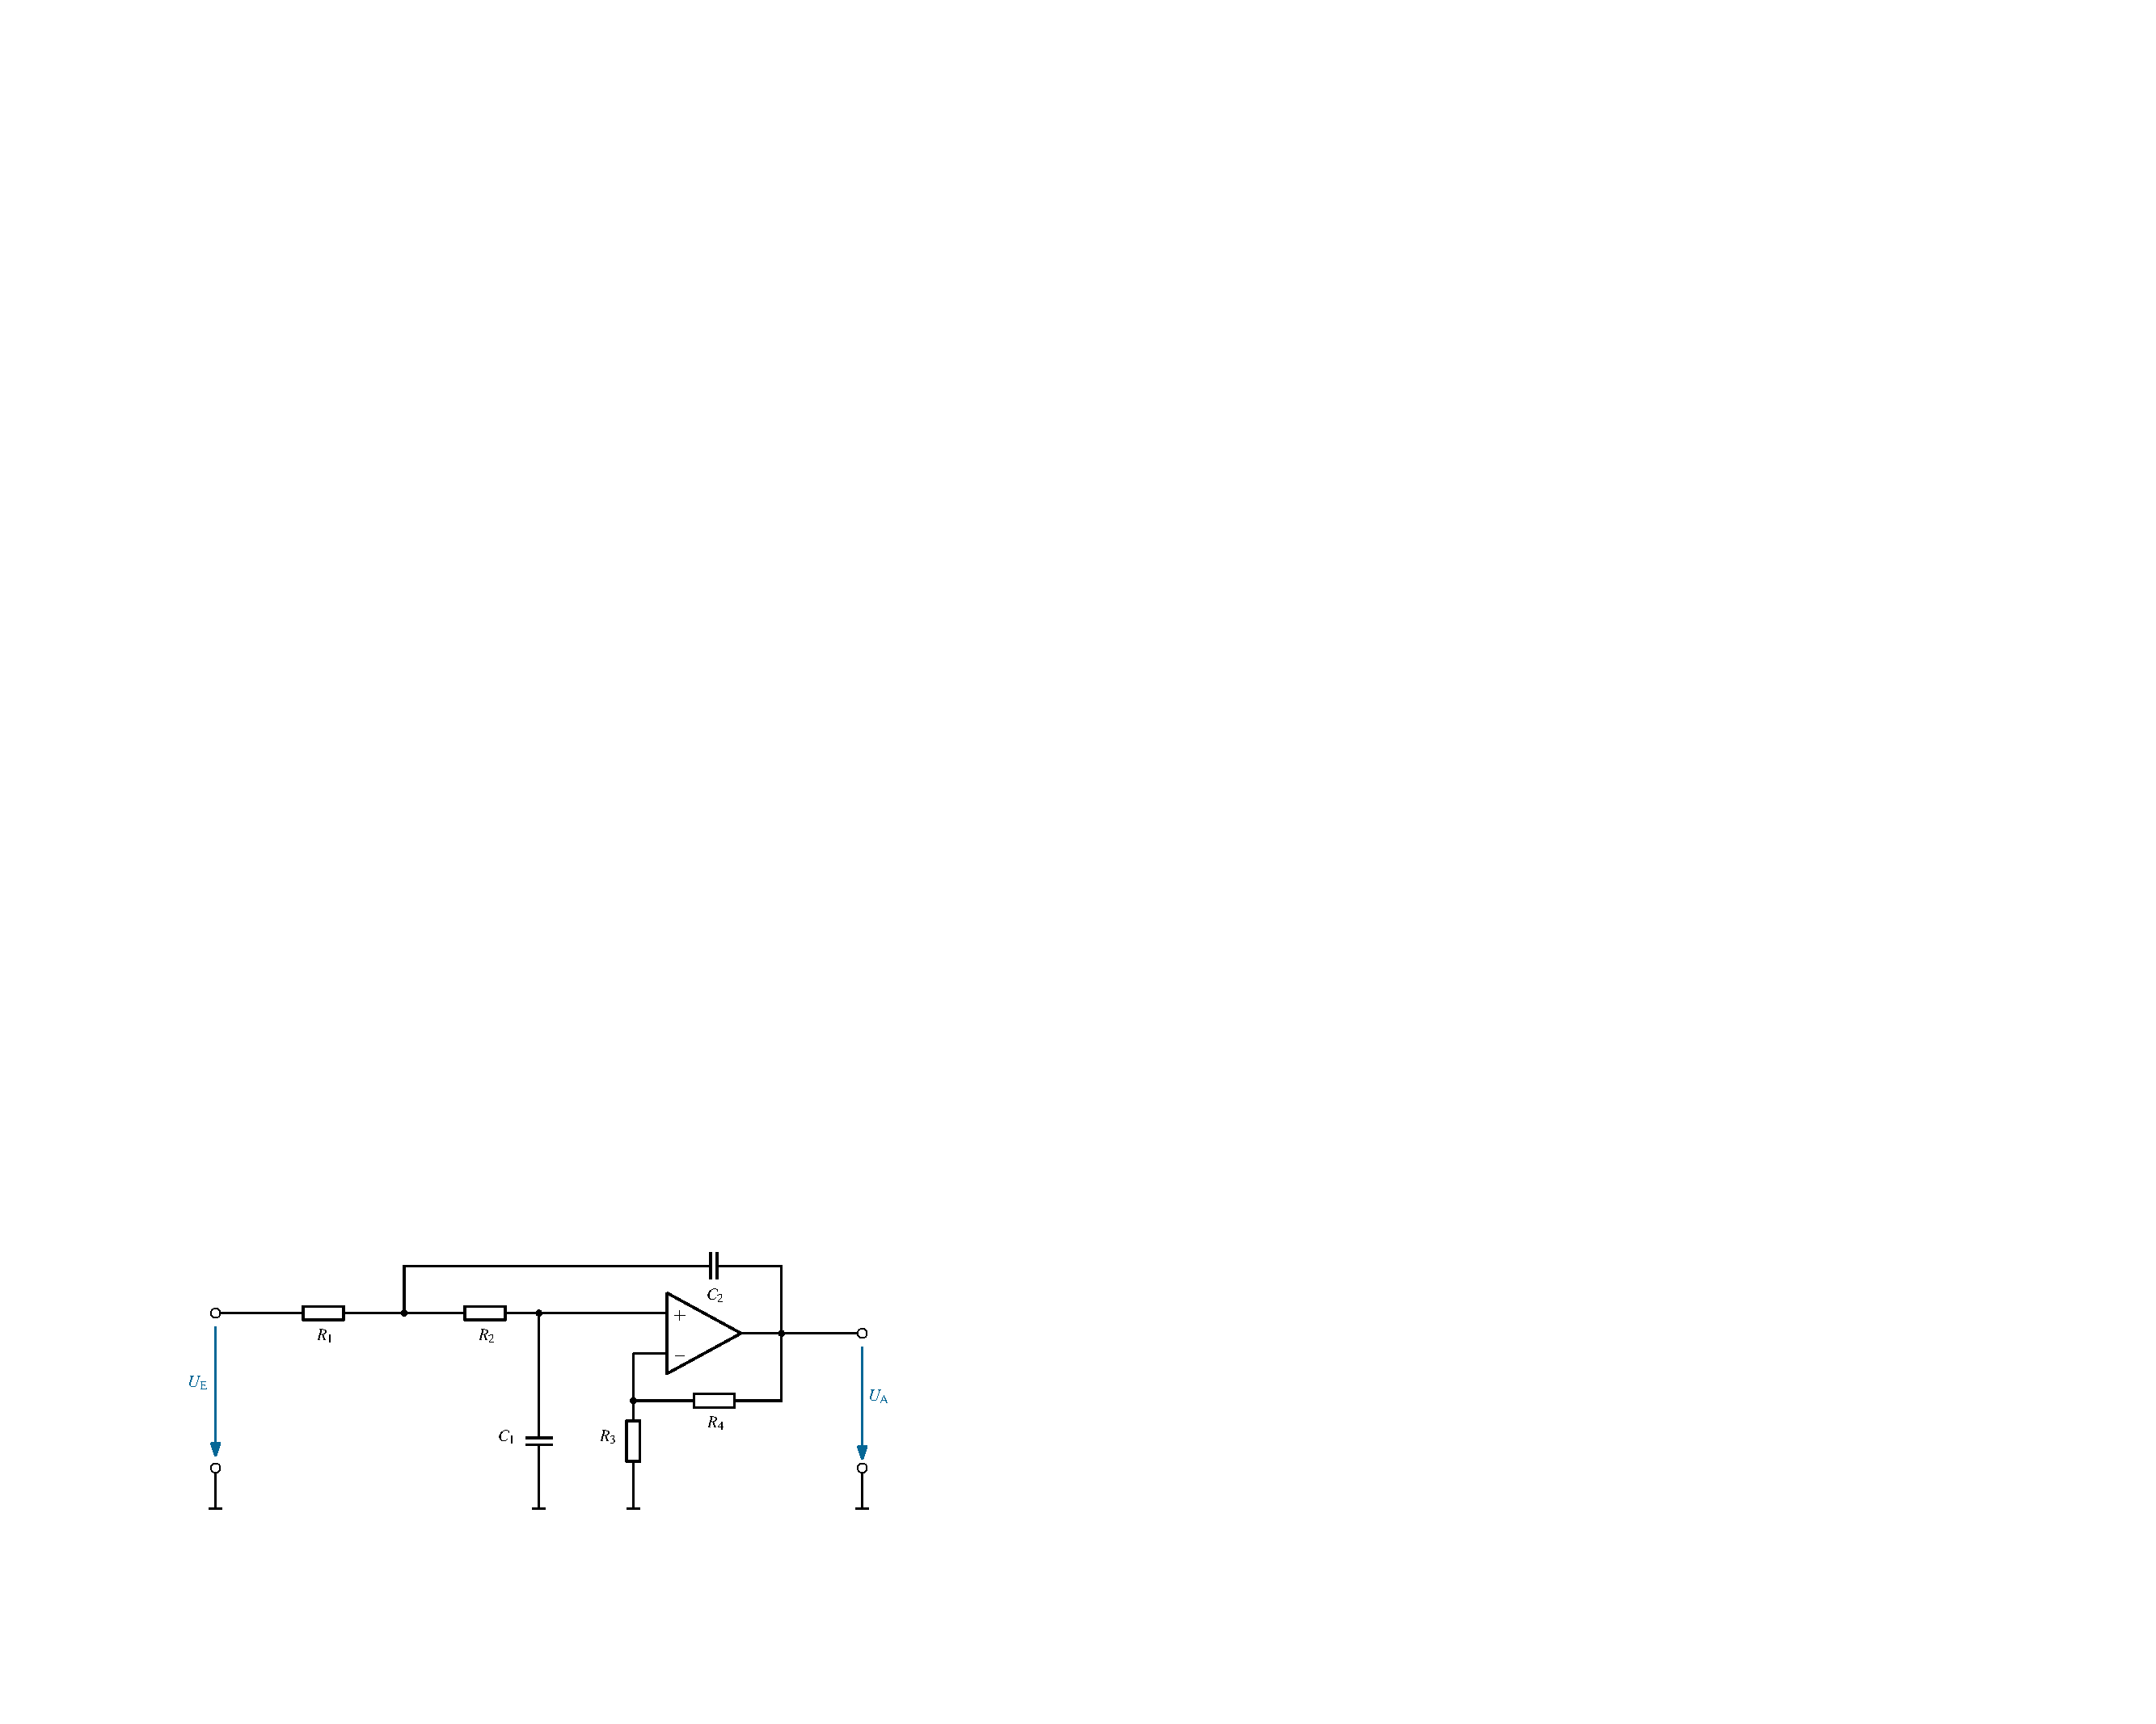
\includegraphics[scale=1]{schaltbild}|  erzugt ein
Bild an der Stelle des Aufrufes:

\begin{lstlisting}
  \begin{center}
    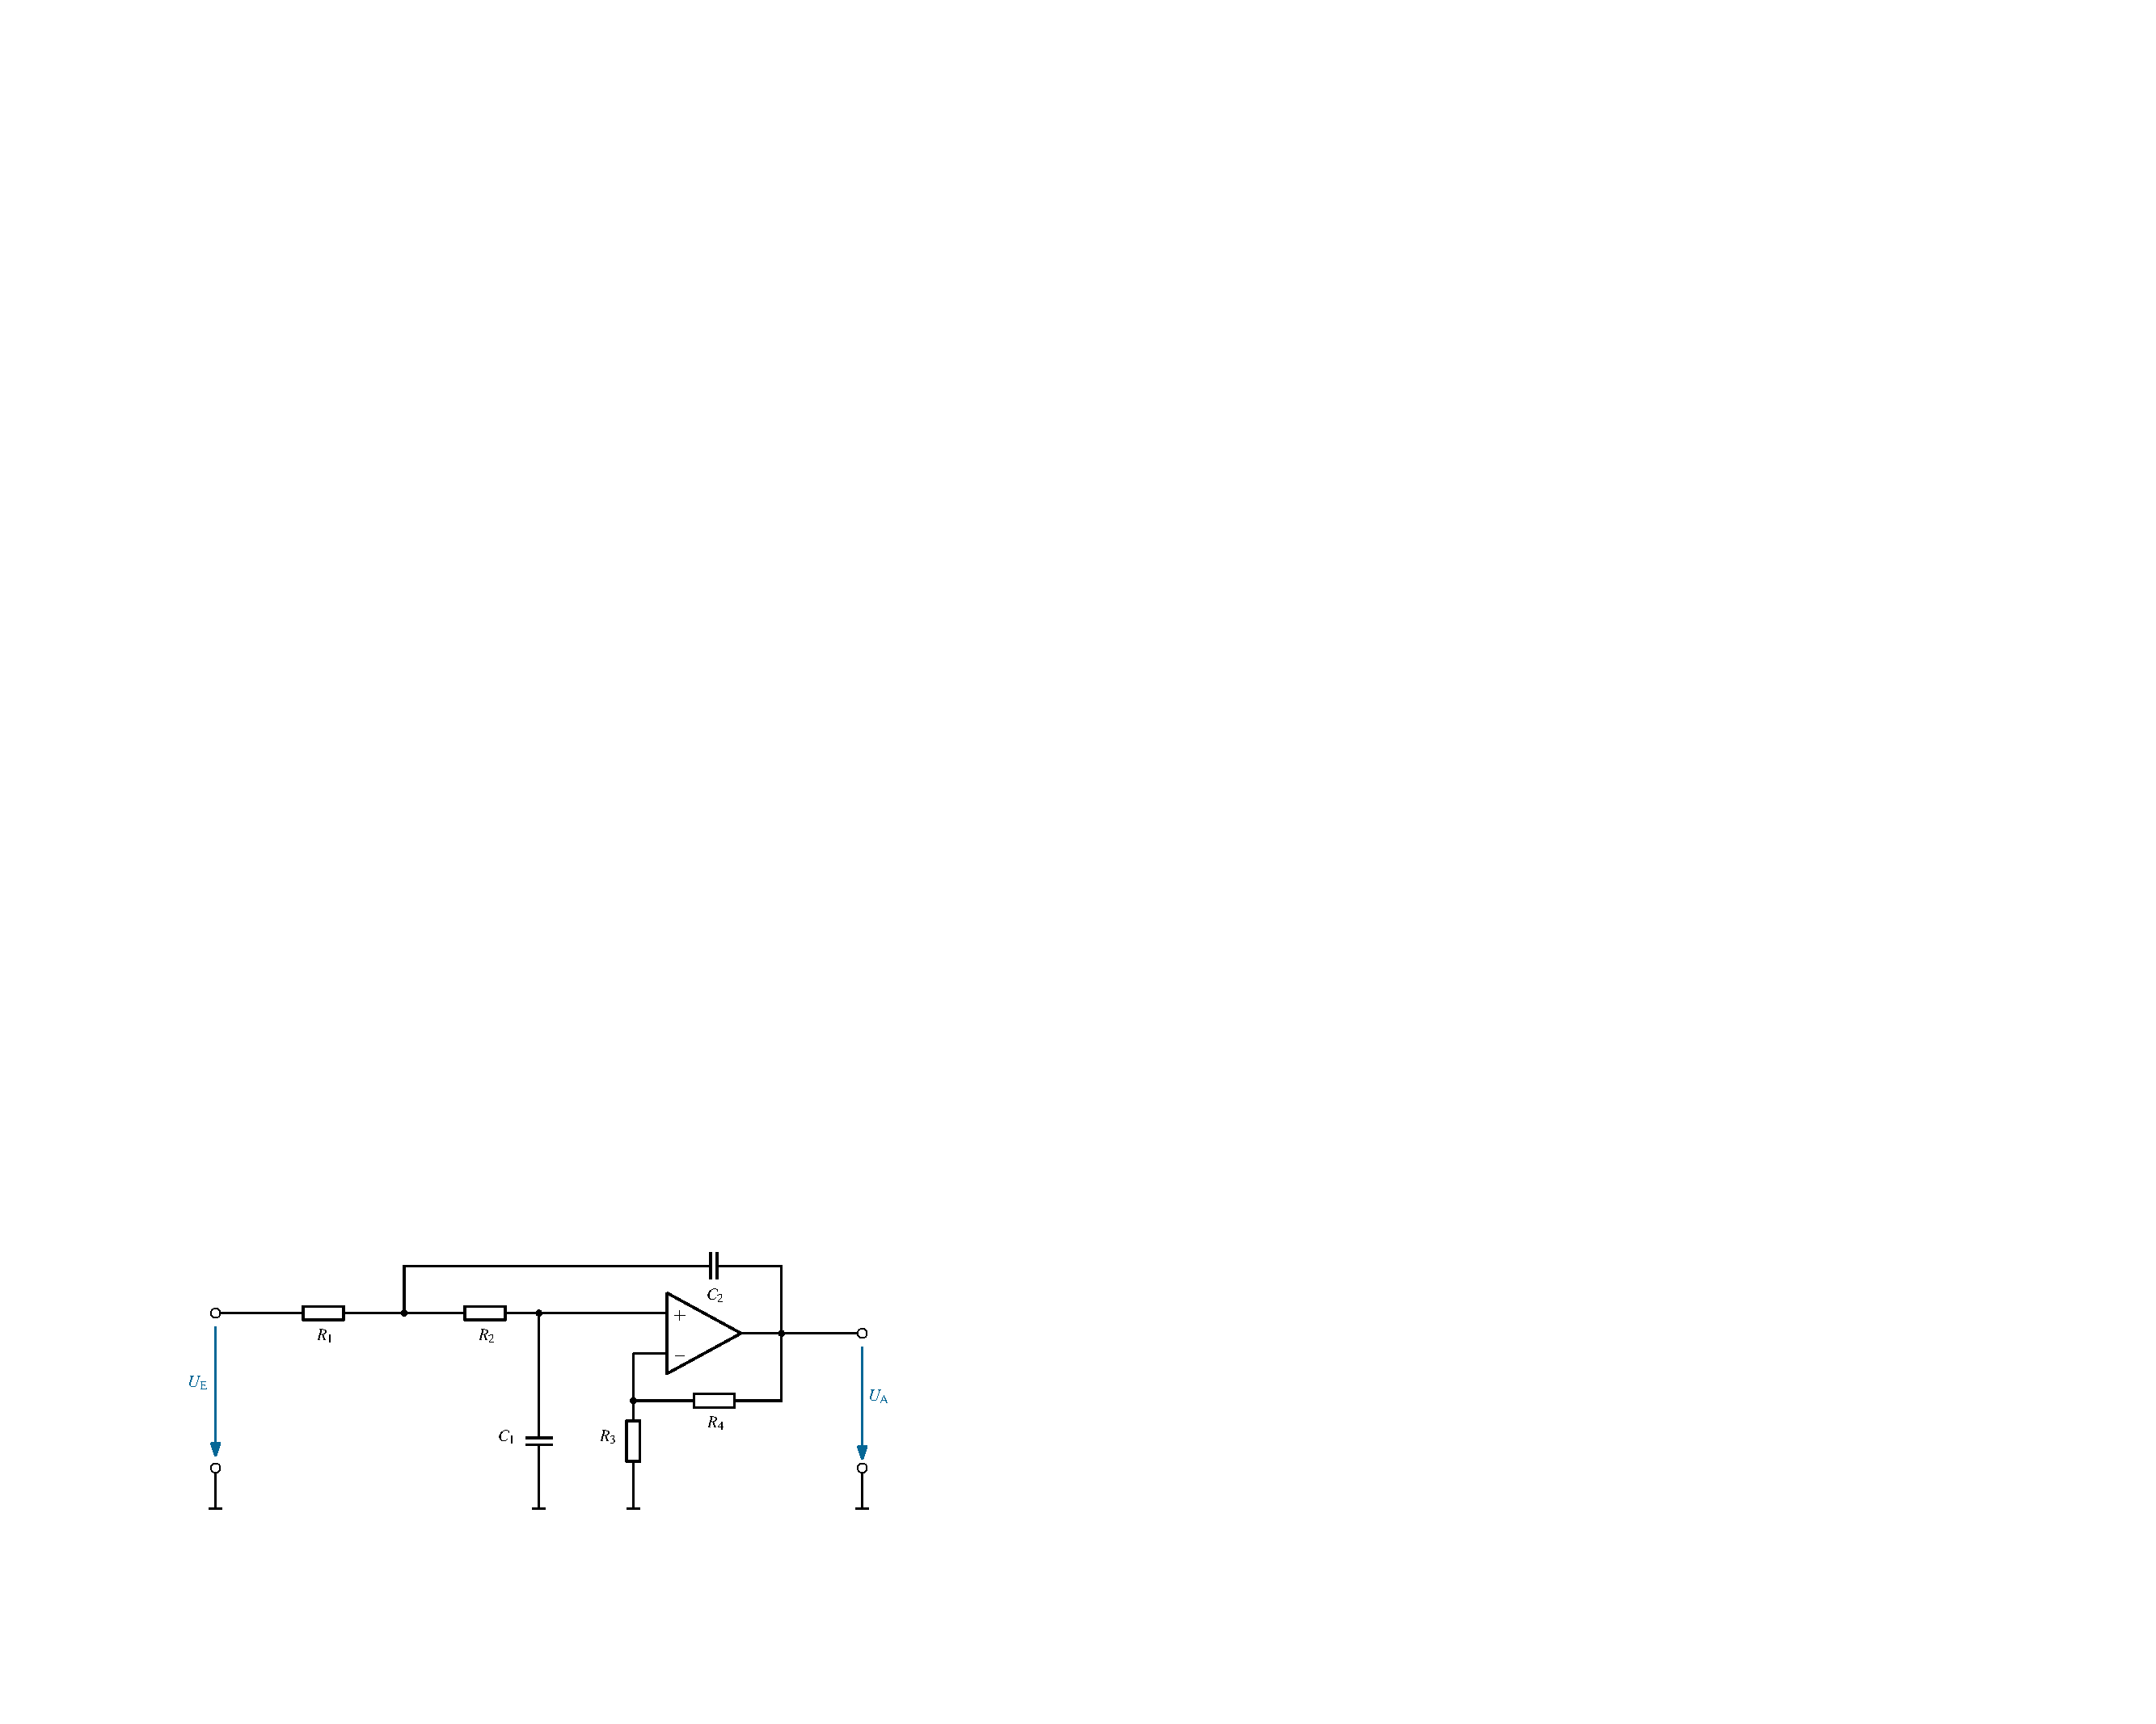
\includegraphics[scale=1]{schaltbild}
  \end{center}
\end{lstlisting}

\begin{center}
  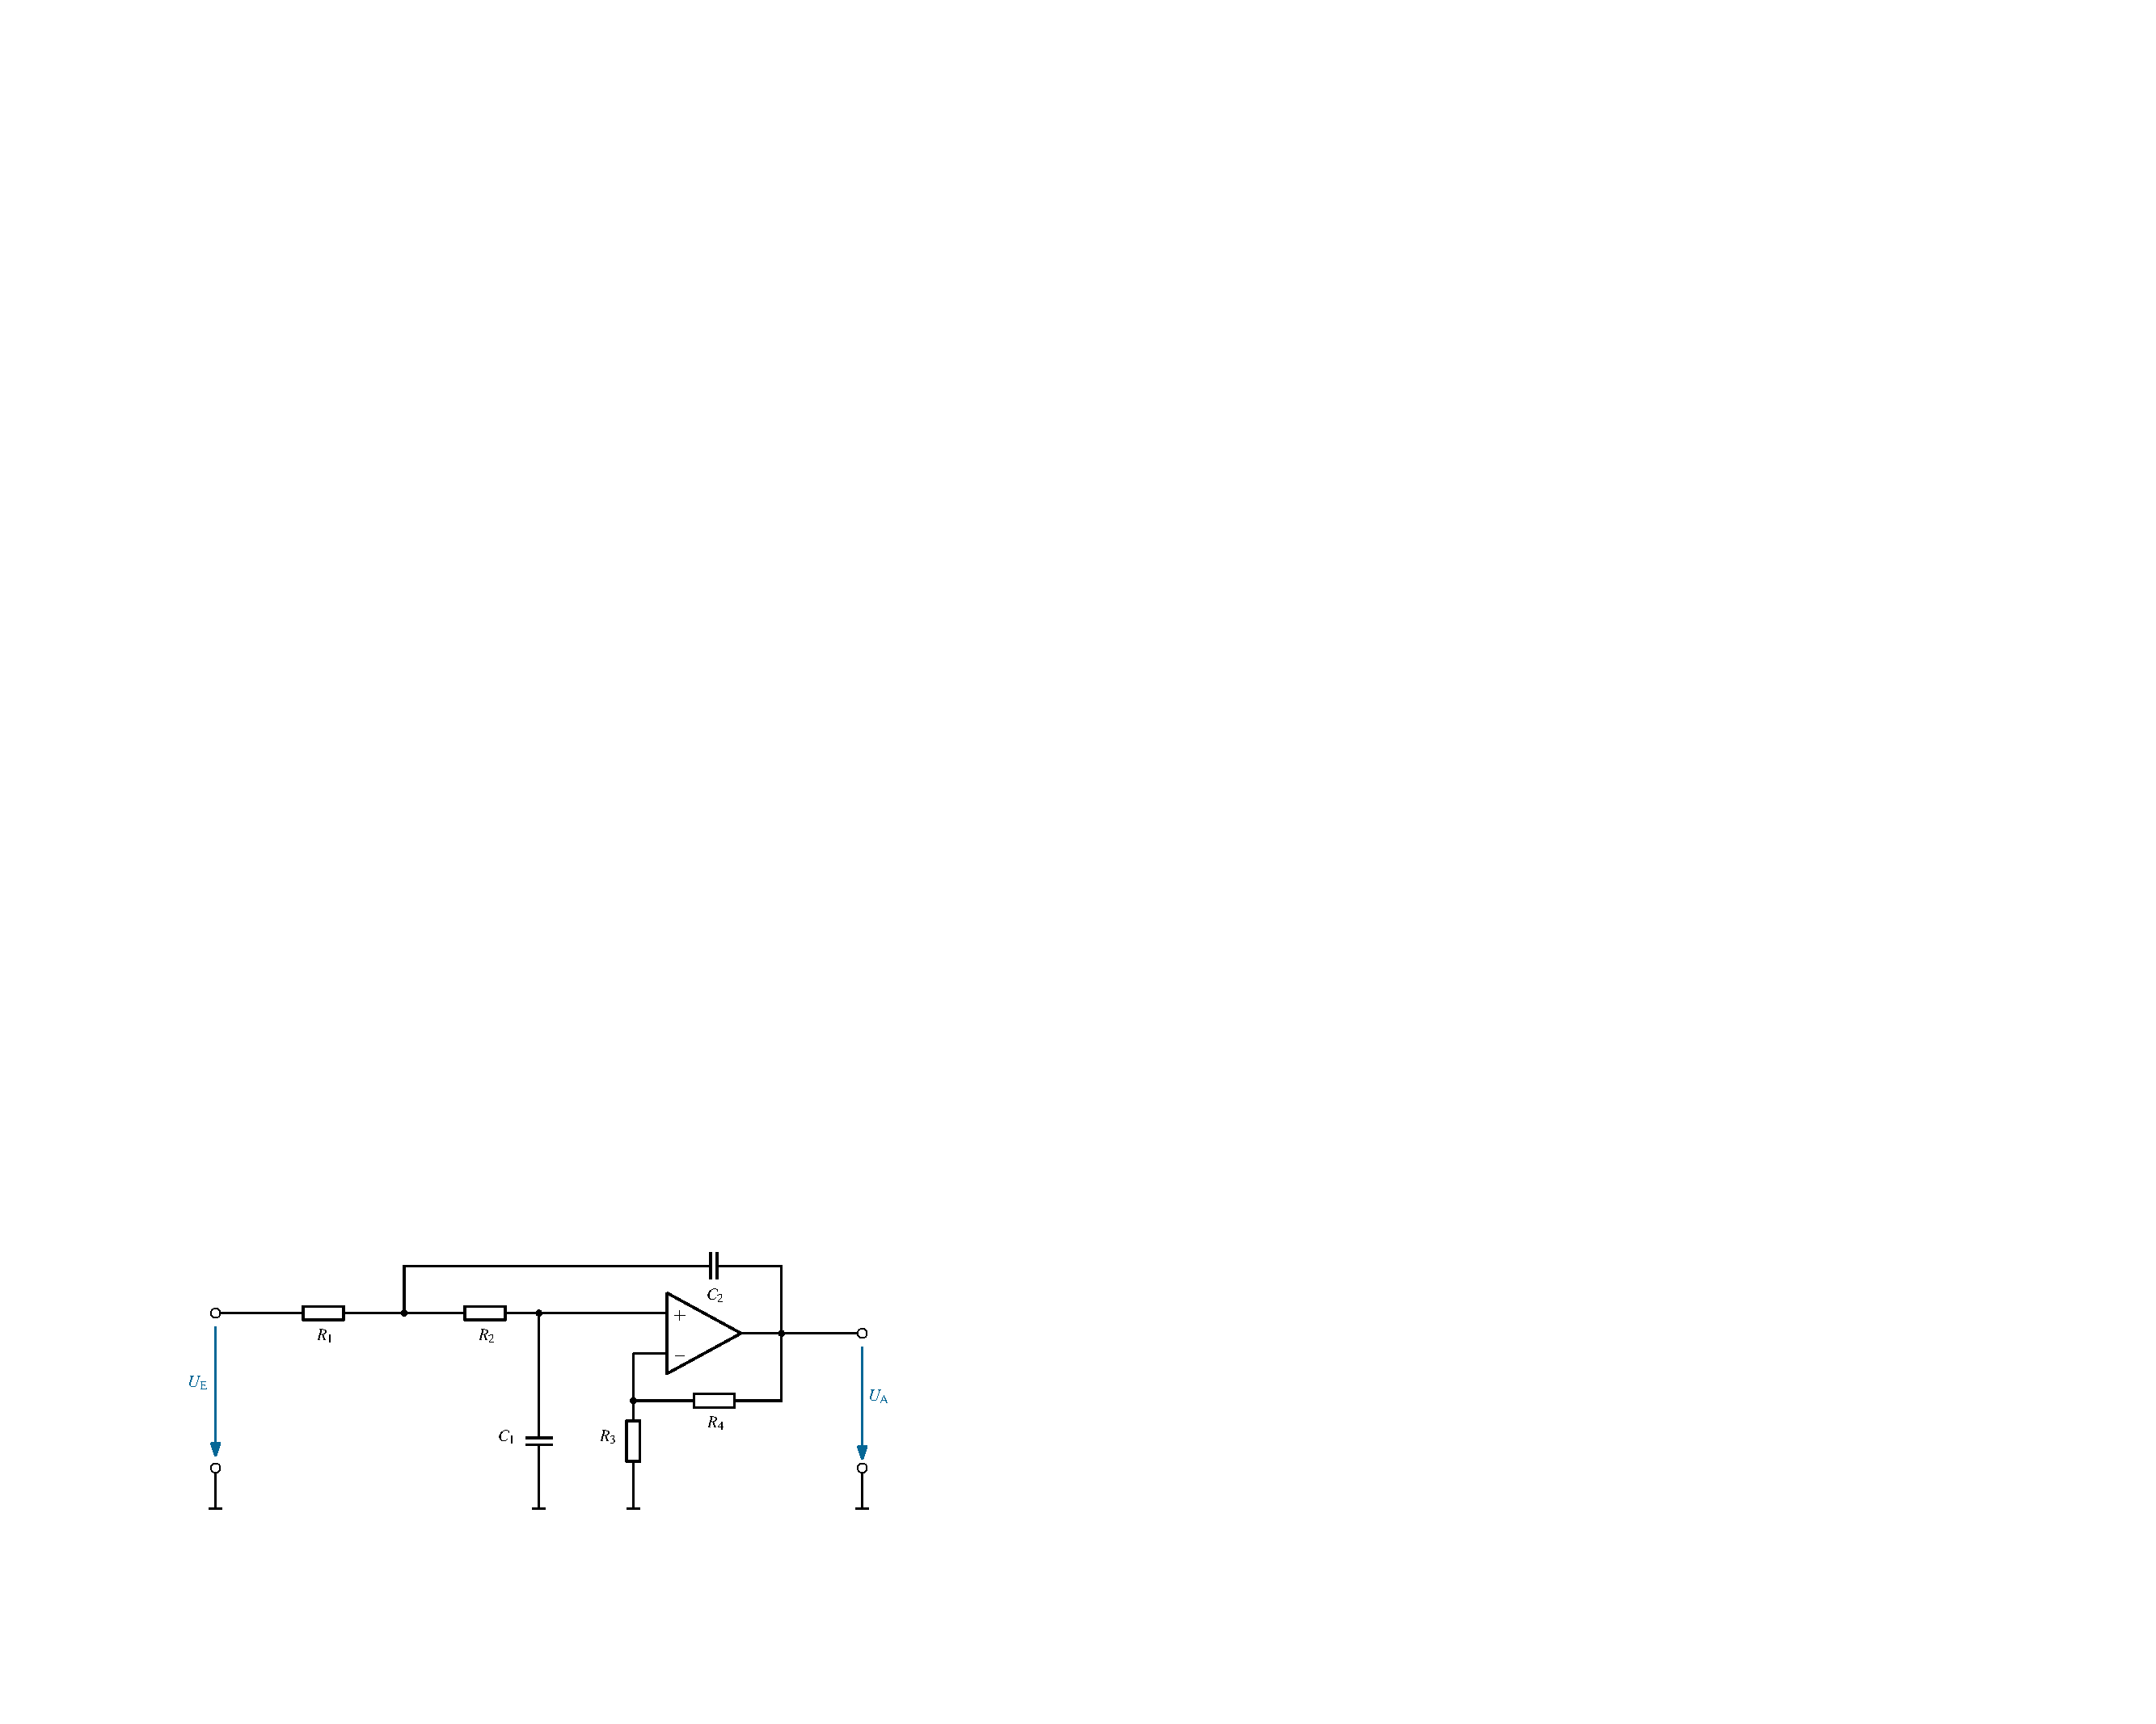
\includegraphics[scale=1]{schaltbild}
\end{center}

Es ist auch möglich, Abbildungen durch den Text \emph{fliessen} zu
lassen. \LaTeX\ kümmert sich um die Positionierung. Das Bild
\ref{fig.Filterschaltung} im Kapitel
\ref{ch.test} wird mit dem Folgenden code erzeugt:

\begin{lstlisting}
\begin{figure}[bht]
  \begin{center}
    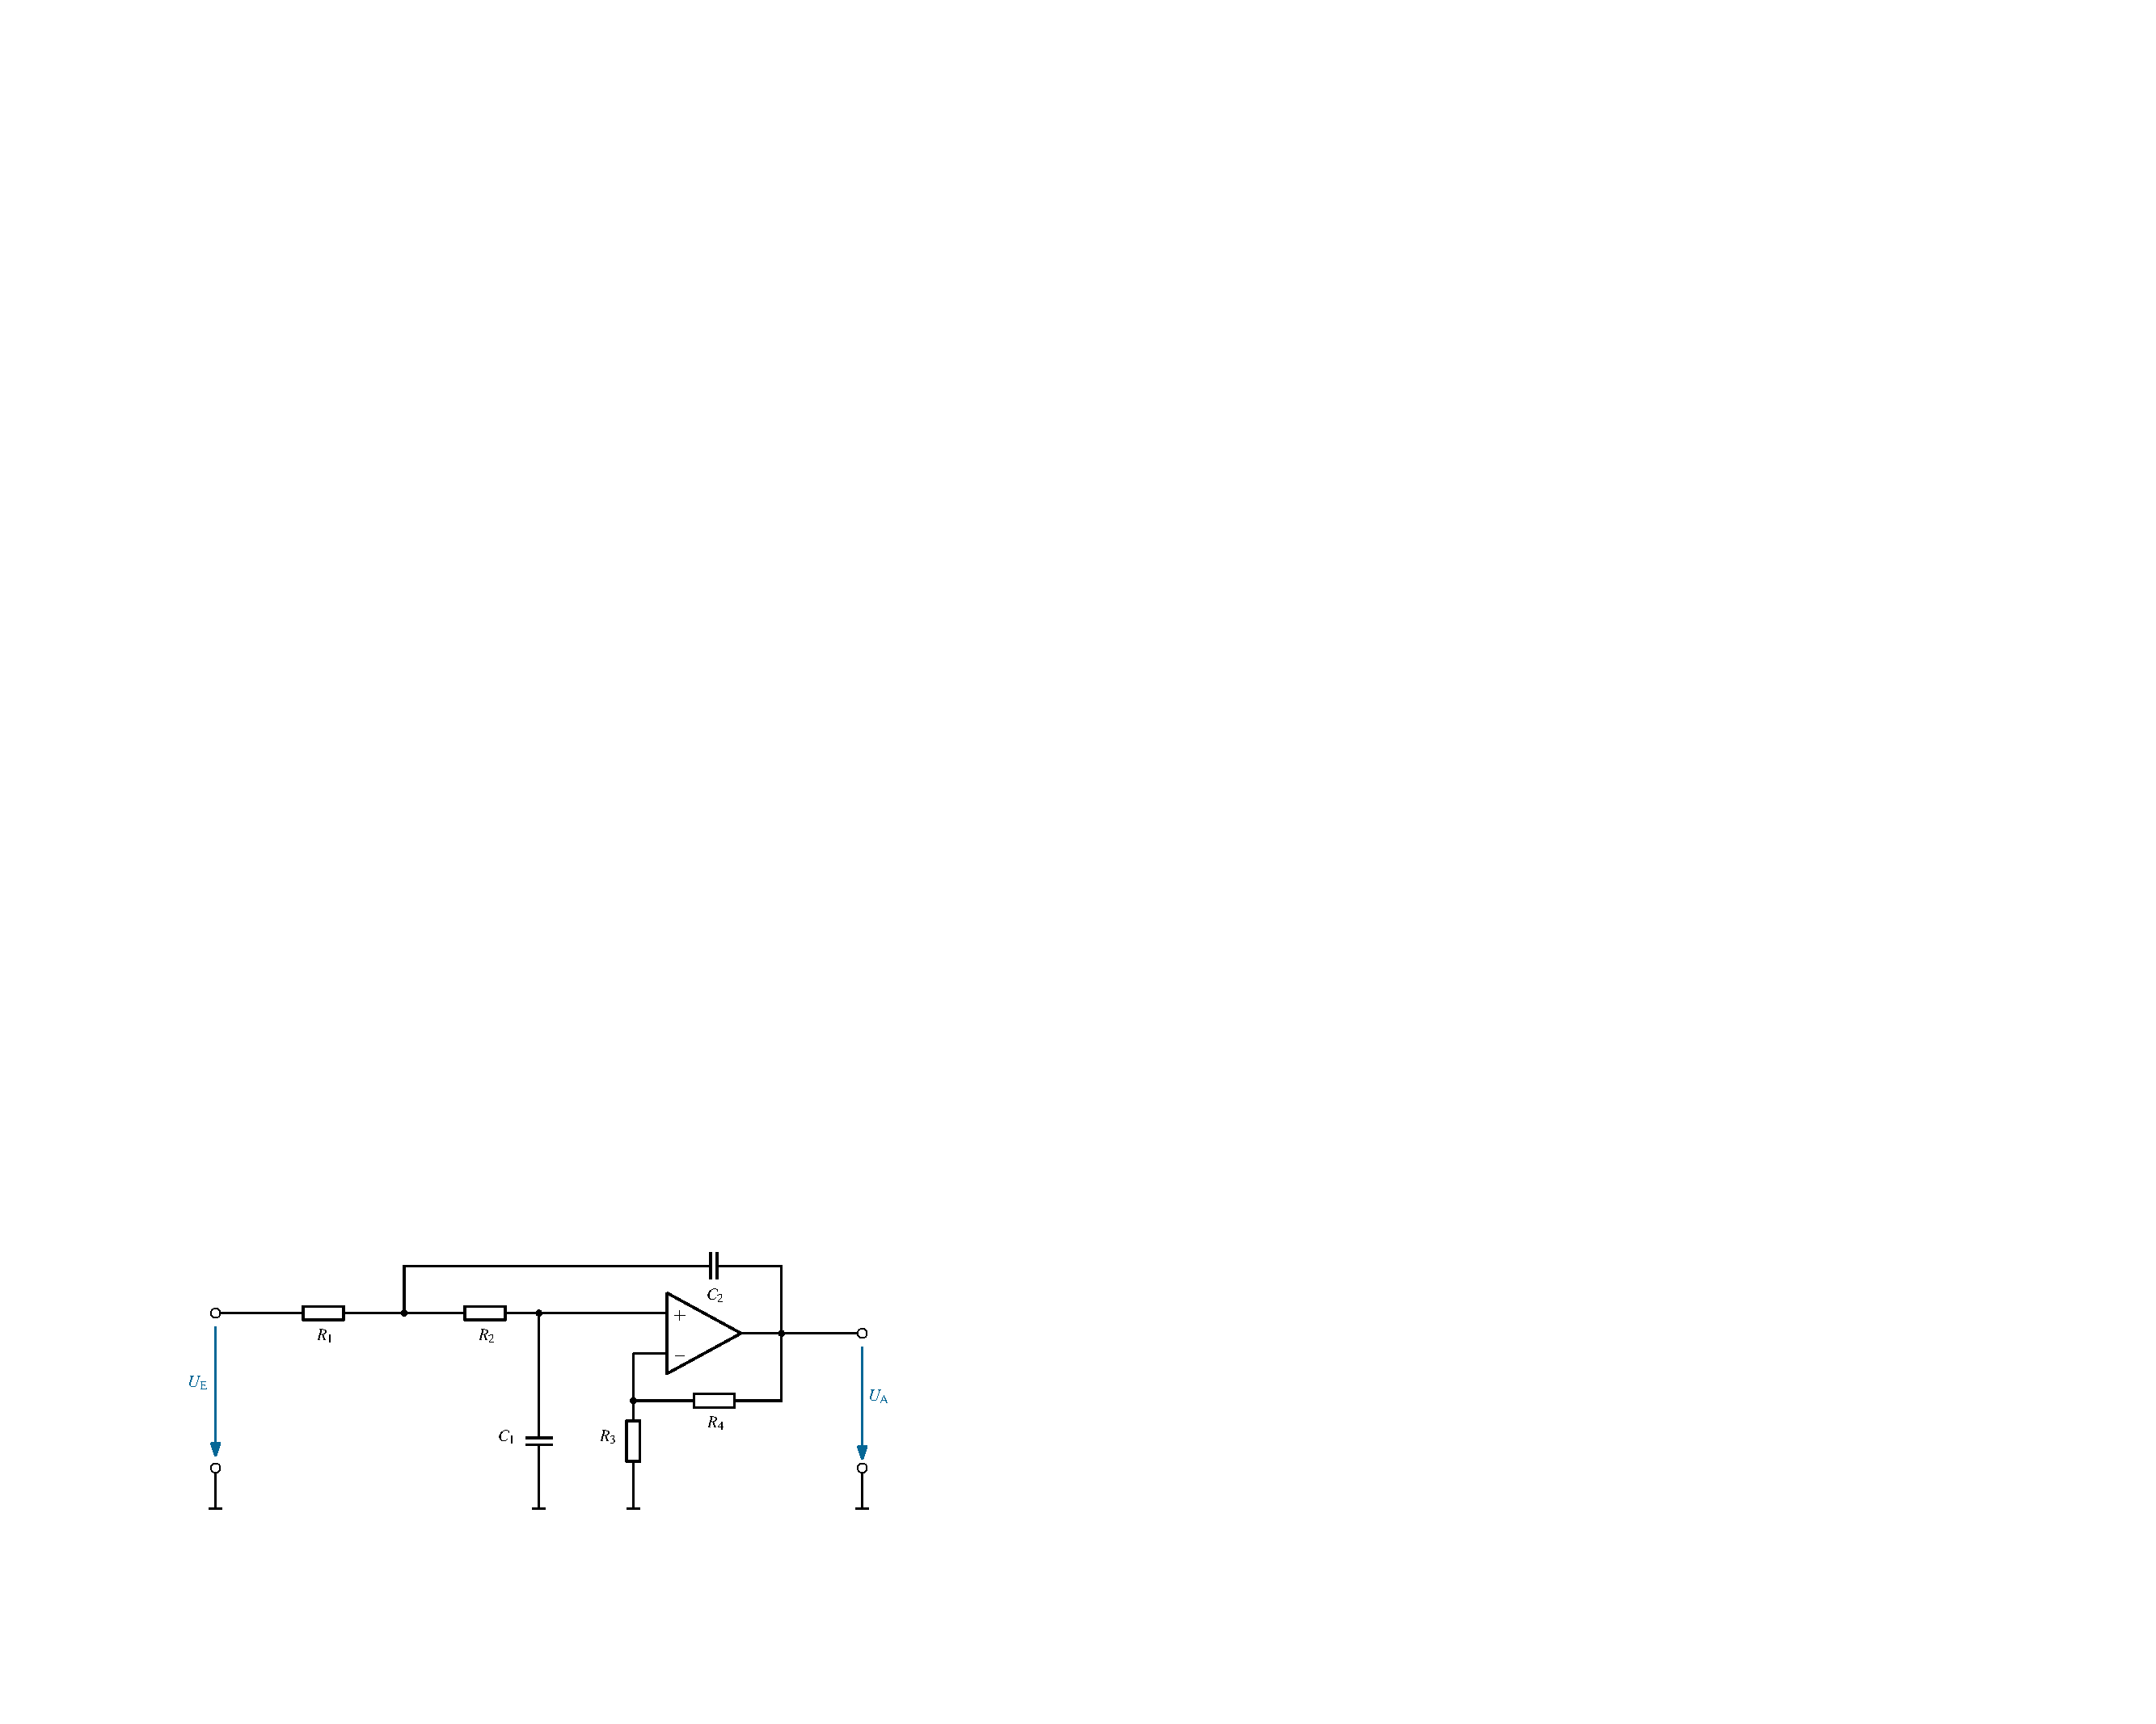
\includegraphics[scale=1]{schaltbild}
    \caption{Die verwendete Filterschaltung}
    \label{fig.Filterschaltung}
  \end{center}
\end{figure}
\end{lstlisting}

Hier ist zu  beachten, dass das Bild auch  automatisch in das Abbildungsverzeichnis
übernommen  wird.  Eine  Referenz  geschieht mit  \verb|\ref{fig.Filterschaltung}|.
Weiterhin braucht  \LaTeX\ etwas Text,  um Bilder darin \emph{fliessen}  zu lassen.
Jegliche Feinabstimmung sollte am Ende nach dem Schreiben des Textes passieren.


\section{Nützliches}

Der Textsatz kann durch viele Pakete in seiner Funktionalität erweitert
werden. Einige seien hier angeführt.

\paragraph{Transfomationssymbole}
Das Paket \texttt{trsym} definiert die Transformationssymbole fu Laplace- und
Fouriertransformation, wie Sie in einigen Lehrbüchern üblich sind.
\begin{equation}
  f(t)\,\TransformHoriz\,F(j\omega)
\end{equation} 
Viele   weitere  Symbole   und   deren  Möglichkeit   zur   Einbindung  werden   in
\cite{latex.symbols} beschrieben.

\paragraph{Querverweise anzeigen}
Das Paket \texttt{showkeys} zeigt alle  in Querverweisen verwendeten Marken im Text
an, so dass Fehler schneller gefunden werden können. 


%% \begin{bytefield}[boxformatting={\centering\itshape},
%%                   bitwidth=1.5em]{20}
%%   \bitheader[b]{0-19}   \\
%%   \bitbox{1}{\tiny F/E} & 
%%   \bitbox{1}{\tiny T0}  & 
%%   \bitbox{1}{\tiny T1}  & 
%%   \bitbox{1}{\tiny Fwd} & 
%%   \bitbox{16}{Data value} \\
%% \end{bytefield}
